\section{Piecewise Hybrid Quadratic Model with Hyperparameters}

When looking at the cobweb diagrams in \Cref{fig:setup.quad.hyper.2.cobwebs}, one can see that the branches $f_\B$ and $f_\D$ are mostly monotonous.
Even when the branches are not, the stable cycles at these points only have points on the monotonously increasing part of these branches.
In this section, we will simplify the model of the previous section by replacing $g_R$, and therefore $f_\B$ and $f_\D$, with a linear function.

\subsection{Model Definition}

The hybrid model is defined as the map $x_{n+1} = f(x_n) \mod 1$.
Where $f$ is given by the following collection of equations.
\begin{align}
	f(x) & = \begin{cases}
		         g(x)                             & \text{if } x < \frac{1}{2} \\
		         g(x - \frac{1}{2}) + \frac{1}{2} & \text{else}
	         \end{cases} \label{equ:quad.full.f}           \\
	g(x) & = \begin{cases}
		         g_L(x) = a_L \cdot x^2 + b_L \cdot x + c_L & \text{if } x < \frac{1}{4} \\
		         g_R(x) = b_R \cdot x + c_R                 & \text{else}
	         \end{cases} \label{equ:quad.full.g}
\end{align}

\subsection{Hyperparameters}

Since the function $g_R$ is now linear, we only need two hyperparameters to fit this branch.
We choose the hyperparameters $g_R\left(\frac{1}{4}\right)$ and $g_R\left(\frac{1}{2}\right)$, we ignore the hyperparameter $\left. \frac{d}{dx} g_R(x) \right|_{x = \frac{1}[2}}$.
As before, we fix the hyperparameter $g_R\left(\frac{1}{2}\right) = \frac{1}{2} + \frac{1}{40}$ to be just above the bisector $y = x$.
And we vary the hyperparameter $g_R\left(\frac{1}{4}\right)$.

\begin{subequations}
	\begin{align}
		g_R\left(\frac{1}{4}\right) & = \frac{b_R}{4} + c_R \label{equ:setup.quad.hybrid.A} \\
		g_R\left(\frac{1}{2}\right) & = \frac{b_R}{2} + c_R \label{equ:setup.quad.hybrid.B}
	\end{align}
\end{subequations}

\Crefrange{equ:setup.quad.hybrid.A}{equ:setup.quad.hybrid.B} are the equations for the values of $g_R\left(\frac{1}{4}\right)$ and $g_R\left(\frac{1}{2}\right)$.
This is a system of equations we now need to solve for the parameters $b_R$ and $c_R$.
As before, we simply compute the inverse matrix of the system written as a matrix.
This is shown in \Cref{equ:setup.quad.hybrid.matrix}.

\begin{align}
	\begin{pmatrix}
		\frac{1}{4} & 1 \\
		\frac{1}{2} & 1
	\end{pmatrix}^{-1} & =
	\begin{pmatrix}
		-4 & 4  \\
		2  & -1
	\end{pmatrix}
	\label{equ:setup.quad.hybrid.matrix}
\end{align}

Hence the equations for $b_R$ and $c_R$ in dependence of $g_R\left(\frac{1}{4}\right)$ and $g_R\left(\frac{1}{4}\right)$ are \Crefrange{equ:setup.quad.hybrid.bR}{equ:setup.quad.hybrid.cR}.

\begin{align}
	b_R & = -4 \cdot g_R\left(\frac{1}{4}\right) + 4 \cdot g_R\left(\frac{1}{2}\right) \label{equ:setup.quad.hybrid.bR} \\
	b_R & = 2 \cdot g_R\left(\frac{1}{4}\right) - 1 \cdot g_R\left(\frac{1}{2}\right) \label{equ:setup.quad.hybrid.cR}
\end{align}

\subsection{Behavior}

\todo{Pictures:}

\begin{figure}
	\centering
	\begin{subfigure}{0.4\textwidth}
		\centering
		\includegraphics[width=\textwidth]{50_Quadratic_linearR/2D_Period_Whole/result.png}
		\caption{Full Model}
		\label{fig:quadratic.full.fit.lin.period.full}
	\end{subfigure}
	\begin{subfigure}{0.4\textwidth}
		\centering
		\includegraphics[width=\textwidth]{50_Quadratic_linearR/2D_Period_Whole/result-halved.png}
		\caption{Halved Model}
		\label{fig:quadratic.full.fit.lin.period.halved}
	\end{subfigure}
	\caption{2D Scans of Periods of Adjusted Model...}
\end{figure}

\begin{figure}
	\centering
	\begin{subfigure}{0.3\textwidth}
		\centering
		\includegraphics[width=\textwidth]{50_Quadratic_linearR/Cobweb_A/result.png}
		\caption{At Point A}
		\label{fig:quad.full.fit.lin.CobwebA}
	\end{subfigure}
	\begin{subfigure}{0.3\textwidth}
		\centering
		\includegraphics[width=\textwidth]{50_Quadratic_linearR/Cobweb_B/result.png}
		\caption{At Point B}
		\label{fig:quad.full.fit.lin.CobwebB}
	\end{subfigure}
	\begin{subfigure}{0.3\textwidth}
		\centering
		\includegraphics[width=\textwidth]{50_Quadratic_linearR/Cobweb_C/result.png}
		\caption{At Point C}
		\label{fig:quad.full.fit.lin.CobwebC}
	\end{subfigure}
	\caption{Cobwebs at Different Points}
	\label{fig:quad.full.fit.lin.Cobwebs}
\end{figure}

\begin{figure}
	\centering
	\begin{subfigure}{0.4\textwidth}
		\centering
		\includegraphics[width=\textwidth]{99_Yunus/2D_Period_Zoomed/result.png}
		\caption{Original Model Full}
		\label{fig:quad.final.comparison.og.full}
	\end{subfigure}
	\begin{subfigure}{0.4\textwidth}
		\centering
		\includegraphics[width=\textwidth]{52_Quadratic_linearR_scaled_mirrored/2D_Period_Whole/result.png}
		\caption{Final Model Full}
		\label{fig:quad.final.comparison.fin.full}
	\end{subfigure} \\
	\begin{subfigure}{0.4\textwidth}
		\centering
		\includegraphics[width=\textwidth]{98_Yunus_modpi/2D_Period_Zoomed/result.png}
		\caption{Original Model Halved}
		\label{fig:quad.final.comparison.og.halved}
	\end{subfigure}
	\begin{subfigure}{0.4\textwidth}
		\centering
		\includegraphics[width=\textwidth]{52_Quadratic_linearR_scaled_mirrored/2D_Period_Whole/result-halved.png}
		\caption{Final Model Halved}
		\label{fig:quad.final.comparison.fin.halved}
	\end{subfigure}
	\caption{Comparison of 2D Scans of Periods of Original and Final Model}
	\label{fig:quad.final.comparison}
\end{figure}
